\documentclass[a4paper,10pt]{scrartcl}
\usepackage[ngerman]{babel}
\usepackage[utf8x]{luainputenc}
\usepackage[headsepline,footsepline]{scrpage2}
\usepackage[autostyle=true,german=quotes]{csquotes}
\usepackage{graphicx}
\usepackage{eqlist}
\usepackage[left=25mm, right=25mm, top=27.5mm, bottom=40mm]{geometry}
\usepackage{calc}
\usepackage[justification=centering]{caption}
\usepackage{subcaption}
\usepackage{textcomp}
\usepackage{gensymb}
\usepackage{amsmath}
\usepackage{amsfonts}
\usepackage{amssymb}
\usepackage{tabularx}
\usepackage{multirow}
\usepackage{nicefrac}
\usepackage{float}

\usepackage[pdfa,pdfencoding=unicode]{hyperref}
\usepackage[ngerman,noabbrev]{cleveref}
\usepackage{xcolor}
\hypersetup{
    colorlinks,
    linkcolor={red!50!black},
    citecolor={blue!50!black},
    urlcolor={blue!80!black}
}

% \pdfminorversion=7
\usepackage{xmpincl}

\setlength{\headheight}{15mm}

\clearscrheadfoot
\lohead{
\includegraphics[height=1cm]{include/Logo_TU_Ilmenau.pdf}}
\cohead{Anleitung für den Linienscanner}
\rohead{Version \\ \parbox{\widthof{Version}}{\centering{1.1}}}
\lofoot{\vspace*{-3mm}TU Ilmenau, Fakultät MB, FG Qualitätssicherung und Industrielle Bildverarbeitung}
\cofoot{}
\rofoot{\vspace*{-3mm}\pagemark}
\pagestyle{scrheadings}

% opening
\title{Anleitung\\Linienscanner}
\author{\Large Benjamin Buch}
\date{\large \today}

\titlehead{
Technische Universität Ilmenau\\
Fakultät für Maschinenbau\\
Fachgebiet Qualitätssicherung und Industrielle Bildverarbeitung\\
Univ.-Prof. Dr. rer. nat. Gunther Notni
}

% Ausrichtung der description-Umgebung
\let\description=\eqlist
\let\enddescription=\endeqlist
\let\eqlistlabel\descriptionlabel

\renewcommand{\arraystretch}{1.5}

\begin{document}

\maketitle

\begin{center}
\begin{minipage}{0.6\textwidth}
\begin{description}
  \large
  \item[Autor $\ \ $] Benjamin Buch
  \item[Telefon] 03677~/~69~-~3975\\(Betreuer Dr.-Ing. Andreas Breitbarth)
  \item[E-Mail] benni.buch@gmail.com\\(andreas.breitbarth@tu-ilmenau.de)
\end{description}
\end{minipage}
\end{center}

\bigskip

\begin{abstract}
Der Linienscanner ist ein Messgerät zur 3D-Rekonstruktion. Der Arbeitsplatz
besteht aus dem Messgerät und einem PC mit Monitor, Maus und Tastatur. Das
Messgerät bestehend aus einem Linienlaser, einer 8-Bit-Grauwert-Kamera, sowie
einem XYZ-Verschiebetisch mit 2 Drehachsen, welche durch 2 MCL Boxen angesteuert
werden.
\end{abstract}

\bigskip

\begin{center}
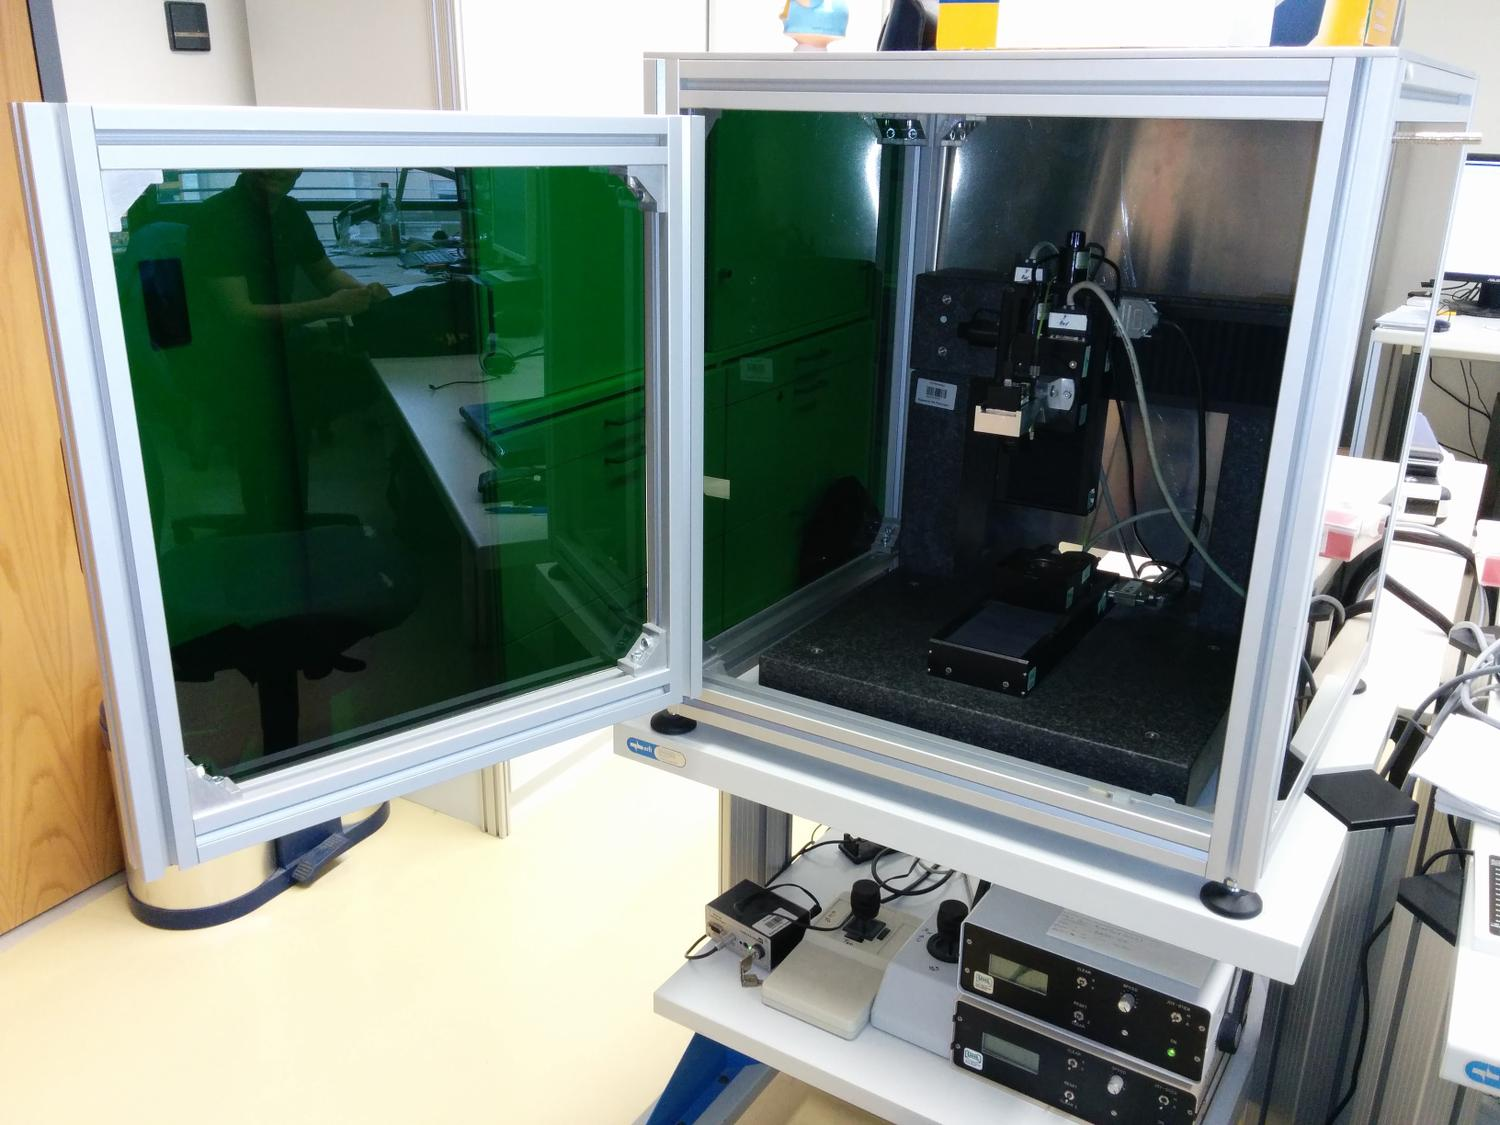
\includegraphics[width=0.7\textwidth]{include/IMG_20160412_140245.jpg}
\end{center}

\section{Begriffe und Definitionen}

Im vorliegenden Dokument werden 2D-Koordinaten mit Kleinbuchstaben (x, y) bezeichnet.
Für 3D-Koordinaten werden Großbuchstaben (X, Y, Z) verwendet.

\section{Einschalten}

Als Erstes sollte der PC eingeschaltet werden, da das Hochfahren aufgrund der alten Hardware
recht lange dauert (ca. 2 Minuten). Das Einloggen erfolgt über den Gast-Account.

Die Energieversorgung des eigentlichen Messgeräts erfolgt über einen Steckdosen-Verteiler, welcher sich
hinter dem Gerät am Boden befindet. Ausgenommen hiervon ist die Kamera, welche ihren Strom per USB vom
PC bezieht.

Für den Fall, dass Messgerät und PC noch nicht verbunden wurden, erfolgt nachfolgend die Beschreibung
des Anschließens. Mit dem PC verbunden sind ausschließlich die MCL-Boxen (in \cref{fig:Steuerhardware}
mit 2a bezeichnet) sowie die Kamera. Der Linienlaser kann ausschließlich von Hand am Gerät bedient
werden. Die untere MCL-Box steuert den Verschiebetisch in X-, Y- und Z-Richtung, die obere Box ist für
die beiden Drehachsen verantwortlich. Zu beachten ist, dass die für Rotation zuständige Box nicht von der
Software angesteuert wird, sie muss also nicht angeschlossen werden.\footnote{Die Drehachsen sind für den
Messvorgang nicht notwendig und besitzen in Kalibrierrichtung keine Endschalter, wodurch ihre Absolutposition
nicht bestimmt werden kann. Aus Sicherheitsgründen sind sie in der Messsoftware nicht enthalten.}

Von den MCL-Boxen führt je ein Kabel mit serieller Schnittstelle zum PC. Um das Anschließen zu
vereinfachen, werden die Kabel an einen 2-fach-Serial-zu-USB-Adapter angesteckt. Ein weiteres
USB-Kabel führt von der Kamera zum PC. Der PC ist also letztlich über zwei USB-Kabel mit der Hardware
des Messgeräts verbunden.

Nachdem das System hochgefahren wurde und Sie sich im Gast-Account eingeloggt haben, muss das
Messprogramm »linescan« gestartet werden.

\section{Hardware}

\begin{figure}[h]
  \centering
  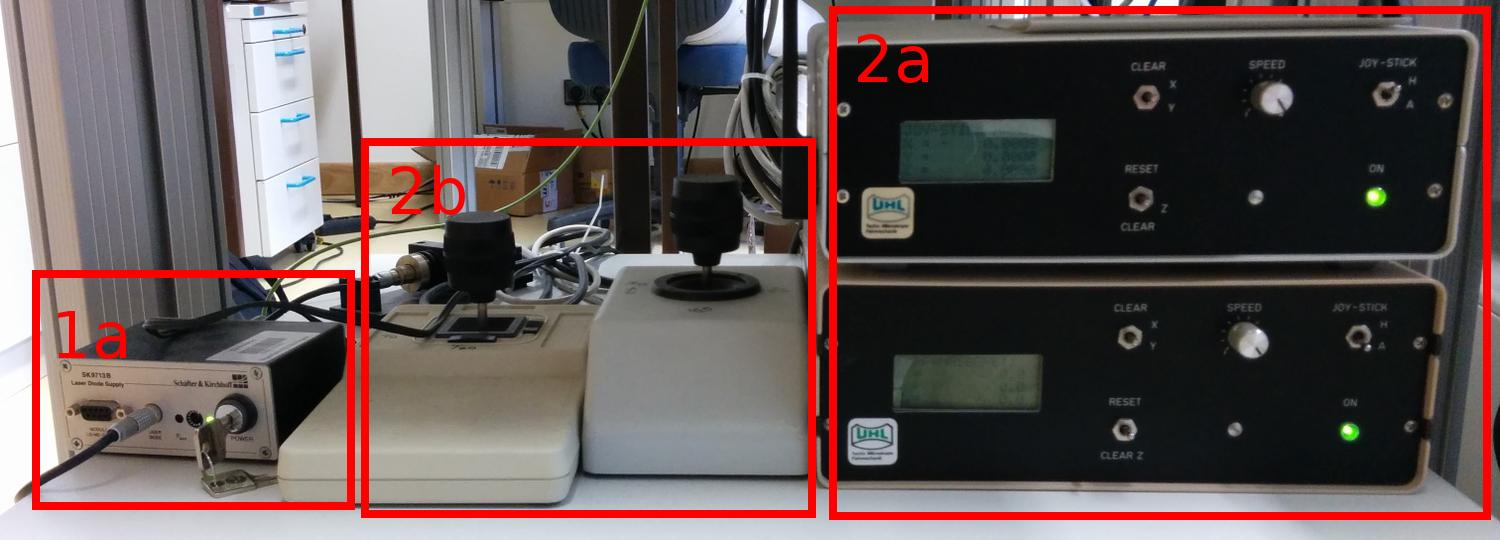
\includegraphics[width=\textwidth]{include/IMG_20160412_140339.jpg}
  \caption{Steuerhardware des Laserliniensystems}
  \label{fig:Steuerhardware}
\end{figure}

\begin{figure}[h]
  \centering
  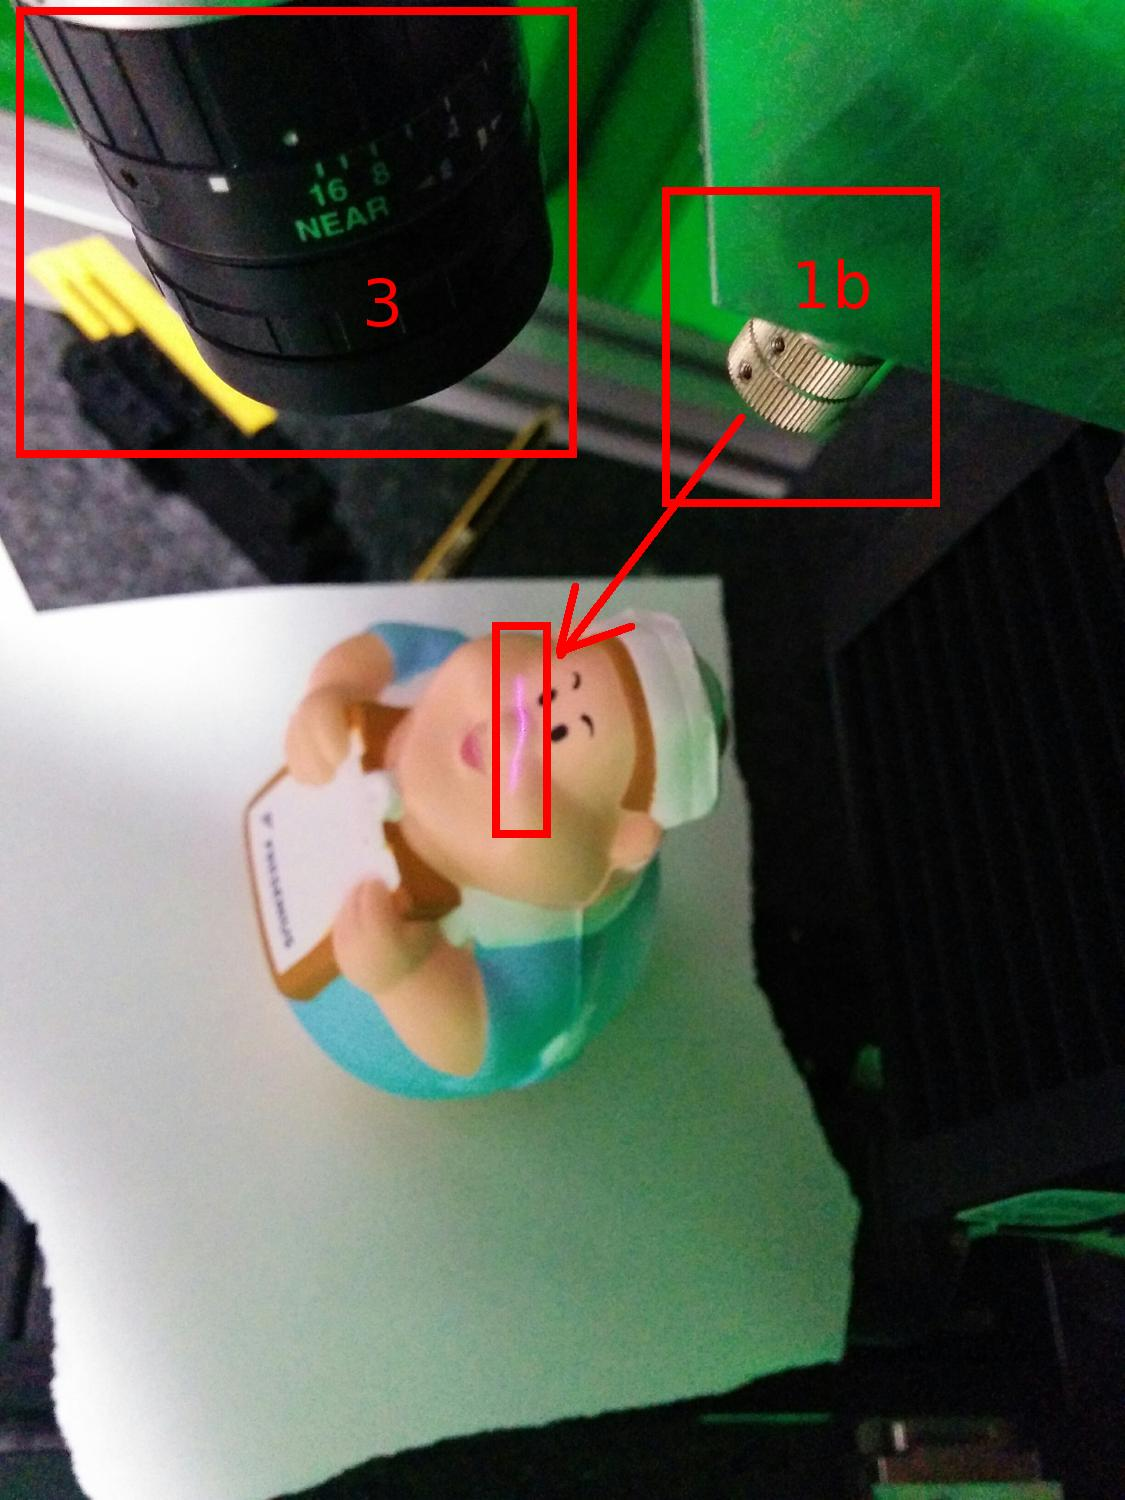
\includegraphics[width=0.5\textwidth]{include/IMG_20160412_135830.jpg}
  \caption{Hardware im Schutzgehäuse sowie beispielhaftes Messobjekt}
  \label{fig:Hardware}
\end{figure}

\newpage
\subsection{Linienlaser}

Über die kleine Box mit dem Schlüssel (\cref{fig:Steuerhardware}, Rahmen 1a) kann der
Linienlaser (\cref{fig:Hardware}, Rahmen 1b) an- und ausgeschaltet werden.
\textit{Vorsicht! Schauen Sie bei aktiviertem Laser nicht ungeschützt in die Lichtquelle.}

\subsection{MCL-Boxen}

Die MCL-Boxen (\cref{fig:Steuerhardware}, Rahmen 2a) können wahlweise per PC (A-Stellung) oder
per Joystick (\cref{fig:Steuerhardware}, Rahmen 2b, H-Stellung) gesteuert
werden. Zur Steuerung der Z-Achse per Joystick, muss der Steuerknüppel gedreht werden. Im Messbetrieb
ist immer die Steuerung über den PC (A-Stellung) notwendig.

\subsection{Kamera}

Die Kamera (\cref{fig:Hardware}, Rahmen 3) wird ausschließlich von der Messsoftware am PC angesteuert.

\newpage

\section{Messsoftware}

\subsection{Kalibriermodus}

\begin{figure}[H]
  \centering
  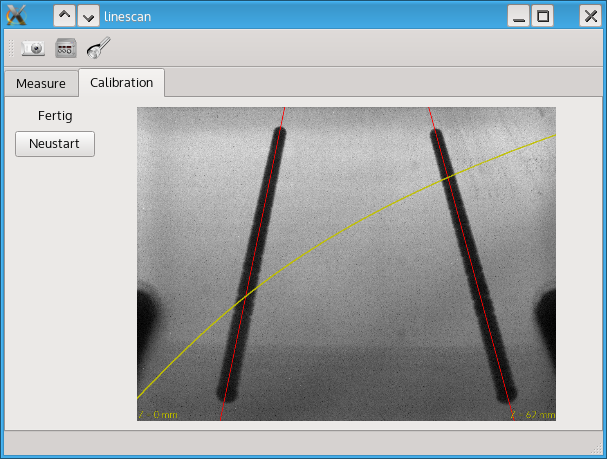
\includegraphics[width=0.5\textwidth]{include/calib.png}
  \caption{Ergebnis einer Systemkalibrierung, Erleuterung in \cref{sec:Kalibrierung}}
  \label{fig:Kalibrierung}
\end{figure}

Im Kalibriermodus (Programm-Reiter »Calibration«) erfolgt die Kalibrierung des Systems.
Messungen können erst durchgeführt werden, wenn eine gültige Kalibrierung existiert.
Ist dies nicht gegeben, sind alle Parameter im Programm-Reiter »Measure« ausgegraut/deaktiviert.
Die Kalibrierung wird auf der Festplatte gespeichert.

\subsection{Messmodus}

\begin{figure}[H]
  \centering
  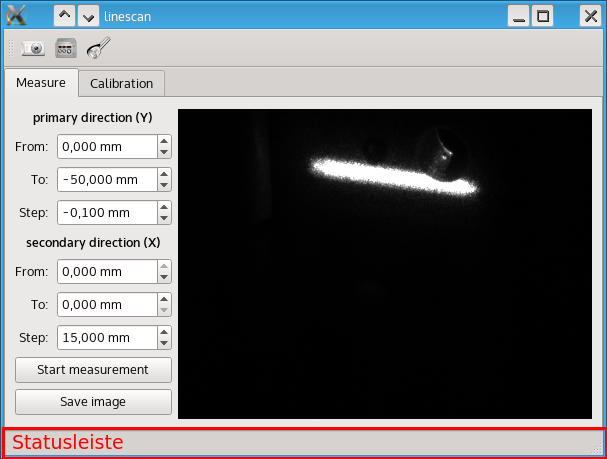
\includegraphics[width=0.5\textwidth]{include/measure.png}
  \caption{Messmodus}
  \label{fig:Messmodus}
\end{figure}

Der Messmodus (Programm-Reiter »Measure«) ist die Hauptkomponente des Programms »linescan«.
Dem Prinzip eines Linienscanners folgend,
wird für die Messung ein Bild mit der Laserlinie auf dem Messobjekt aufgenommen. Das Bild wird
in eine Liste von Punkten in der xy-Bildebene der Kamera umgewandelt. Entsprechend der Kalibrierung
werden diese 2D-Punkte in 3D-Punkte transformiert und mit der aktuellen XYZ-Position des
Verschiebetisches (MCL) addiert. Anschließend fährt der Verschiebetisch an die nächste Position,
wo sich der Vorgang wiederholt.

Die Laserebene ist dabei identisch zur XZ-Ebene. Entsprechend erfolgt die Messung primär entlang
der Y-Achse. Um Objekte zu messen, welche breiter als die Laserlinie sind, kann ein sekundäres
Verfahren entlang der X-Achse erfolgen. Wurde das Messfeld in Y-Richtung komplett durchlaufen,
fährt der Tisch an die Y-Startposition und verschiebt das Objekt entsprechend der X-Richtung.
Dann wiederholt sich der Messvorgang in Y-Richtung.

Wurde das Messfeld komplett abgefahren oder die Messung manuell unterbrochen, kehrt der Tisch
in die Startposition zurück und speichert das gemessene Objekt als ASCII-Punktwolke auf der
Festplatte. Der Dateiname wird für ein paar Sekunden in der Statusleiste des Messprogramms
(unten) angezeigt.

\subsection{MCL}

\begin{figure}[H]
  \centering
  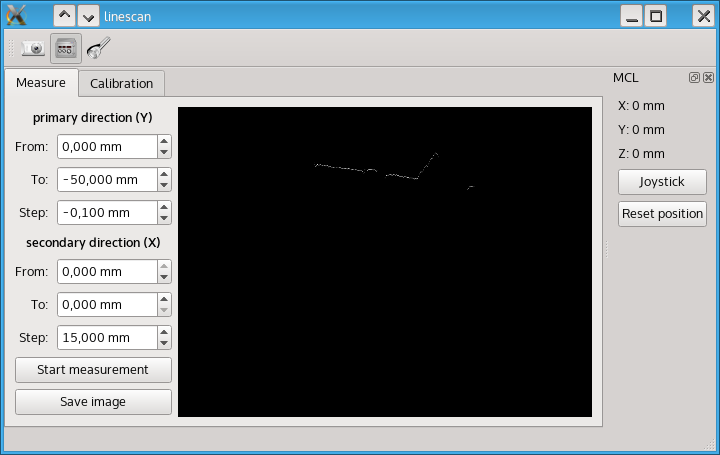
\includegraphics[width=0.5\textwidth]{include/mcl.png}
  \caption{MCL}
  \label{fig:MCL-Dock}
\end{figure}

Das MCL-Dock kann über den entsprechenden Toolbar-Button ein- und ausgeblendet werden.
Hier werden die aktuellen Positionen des XYZ-Verschiebetisches angezeigt. Mittels »Reset Position« kann die Position
hier genullt werden. Außerdem kann die Joysticksteuerung softwareseitig aktiviert werden.

\textsl{Achtung:} Ein manuelles Umschalten an der MCL-Box kann zu Inkonsistenzen führen, welche eine
falsche Skalierung der Messung zur Folge haben!

\newpage
\subsection{Bildeinzug – Parametrisierung}

\begin{figure}[H]
  \centering
  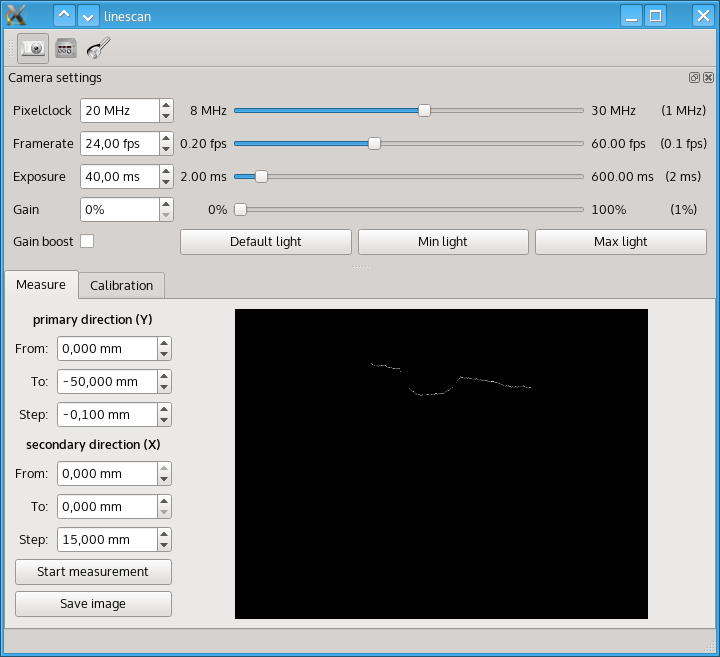
\includegraphics[width=0.48\textwidth]{include/cam.png}
  \caption{Bildeinzug}
  \label{fig:Bildeinzug}
\end{figure}

Das Kamera-Dock kann über den entsprechenden Toolbar-Button ein- und ausgeblendet werden.
Hier sind alle Einstellungen zum Bildeinzug zu finden. Über die drei Buttons »Default light«,
»Min light« und  »Max light« kann eine Schnelleinstellung erfolgen.

\subsection{Linienberechnung}

\begin{figure}[H]
  \centering
  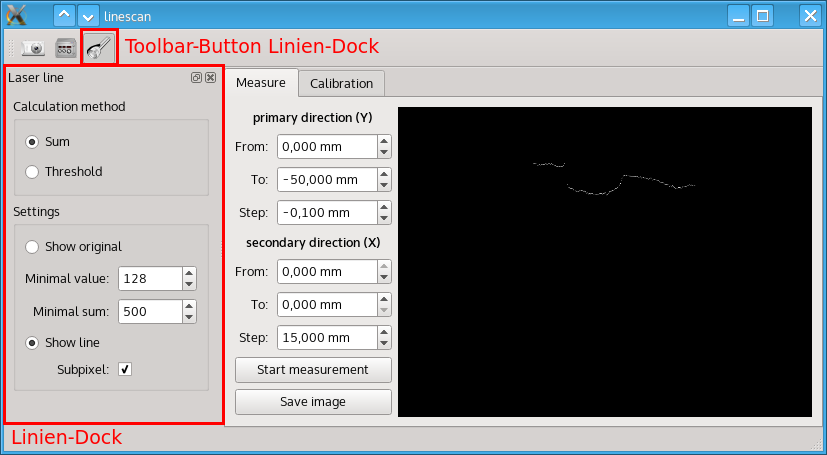
\includegraphics[width=0.5\textwidth]{include/laser.png}
  \caption{Linienberechnung}
  \label{fig:Linienberechnung}
\end{figure}

Das Linien-Dock kann über den entsprechenden Toolbar-Button ein- und ausgeblendet werden.
Hier kann primär die Methode zur Detektion der Linie im Bild (»Sum« oder »Threshold«) gewählt
werden. Darunter kann der gewählte Algorithmus parametriert werden. Zur besseren Veranschaulichung
können die einzelnen Schritte der Algorithmen durch Auswahl des entsprechenden Radio-Buttons
(»Show original« oder »Show line«) dargestellt werden.

\subsubsection{Methoden zur Detektion der Linie im Bild}

Aufgrund der schlechten Qualität des Lasers wird die Laserlinie mit starker Überbelichtung aufgenommen.
In \cref{fig:Messmodus} ist dies zu erkennen. Die Detektion erfolgt immer eindimensional entlang der y-Achse. Die
nachfolgend beschriebenen Methoden werden also für jeden x-Wert einmal durchgeführt, wodurch der zugehörige
y-Wert berechnet wird, falls in y-Richtung die Linie an der aktuellen x-Position detektiert werden konnte.

\paragraph{Methode »Threshold«}

Bei dieser Methode werden zunächst alle Werte entsprechend einem Schwellwert binarisiert. Anschießend
werden zusammenhängende Bereiche aus Werten, welche größer oder gleich dem Schwellwert waren gebildet.
(Im Idealfall sollte es nur einen zusammenhängenden Bereich geben, in der Praxis entstehen jedoch durch
Reflexion und andere Effekte manchmal sekundäre Bereiche.) Die mittlere Position des größten
zusammenhängenden Bereichs wird als y-Koordinate zurückgegeben. War kein Wert größer als
der Schwellwert, so wurde für diese x-Position kein Linienpunkt erkannt.

\bigskip
\begin{minipage}{\textwidth} 
\textbf{Beispiel: Schwellwert 255}

\begin{verbatim}
y-Position Intensitätswerte Binarisiert
         0                0           0
         1                0           0
         2               60           0
         3              255           1 -> y-Pos: 3
         4              255           1             => y = (3 + 5) / 2 = 4.0
         5              255           1 -> y-Pos: 5
         6               30           0
         7                0           0
         8              255           1
         9                0           0
        10                0           0
\end{verbatim}
\end{minipage}

\paragraph{Methode »Sum«}

Wie der Name bereits andeutet, basiert diese Methode auf der Summe der Intensitätswerte. Konkret werden zwei Summen berechnet, die über alle Intensitätswerte und die über die mit der y-Position gewichteten Intensitätswerte. Teilt man Letztere durch Erstere, ergibt sich wieder eine y-Position, welche zurückgegeben wird. Die Summe der Intensitätswerte muss mindestens dem als Parameter übergebenen Schwellwert entsprechen, andernfalls wurde für die aktuelle x-Position kein Linienpunkt erkannt.

\bigskip
\begin{minipage}{\textwidth} 
\textbf{Beispiel: Schwellwert 200}

\begin{verbatim}
y-Position    Intensitätswerte    Gewichtet
         0         ·         0      =     0
         1         ·         0      =     0
         2         ·        60      =   120
         3         ·       255      =   765
         4         ·       255      =  1020
         5         ·       255      =  1275
         6         ·        30      =   180
         7         ·         0      =     0
         8         ·       255      =  2040
         9         ·         0      =     0
        10         ·         0      =     0
                   Summe: 1110  Summe: 5400  => y = 5400 / 1110 = 4.86
\end{verbatim}
\end{minipage}

\newpage
\section{Kalibrierung}
\label{sec:Kalibrierung}

\begin{figure}[H]
  \centering
  $\vcenter{\hbox{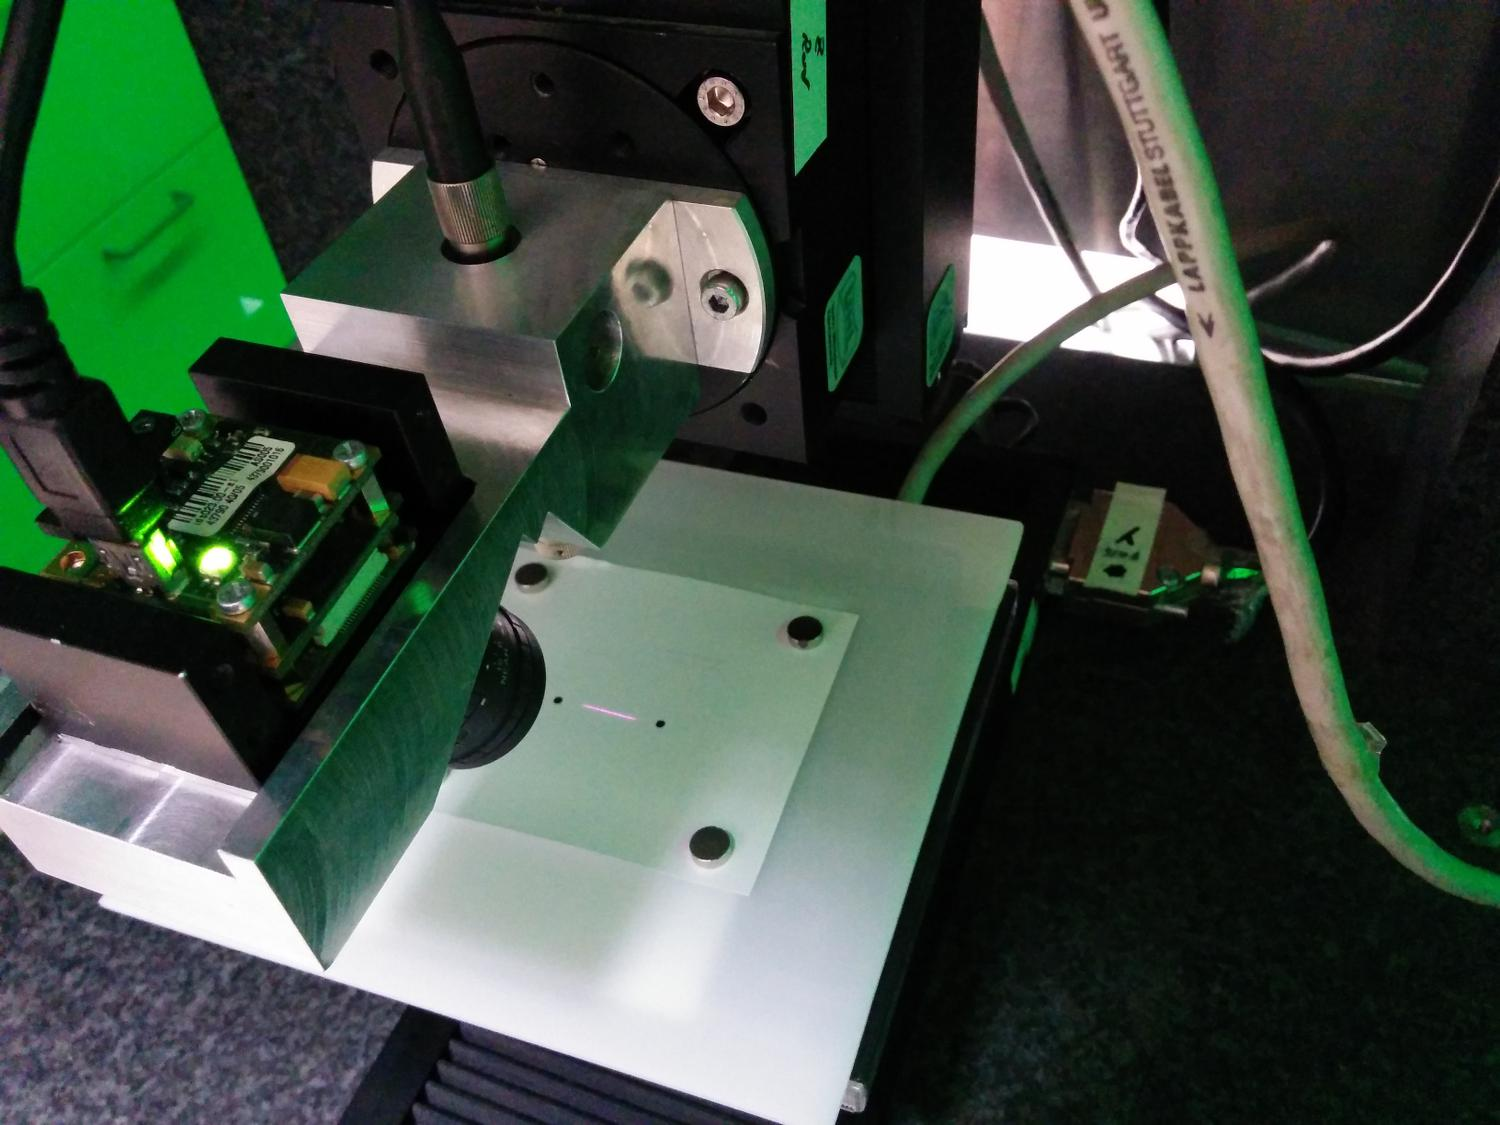
\includegraphics[width=0.45\textwidth]{include/IMG_20160412_162021.jpg}}}$
  \hspace*{1cm}
  $\vcenter{\hbox{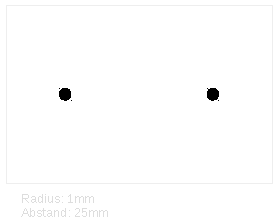
\includegraphics[width=0.3\textwidth]{include/target.pdf}}}$
  \caption{Kalibriertarget während eines Kalibriervorgangs im Messsystem (links), Kalibriertarget (rechts)}
  \label{fig:Kalibriertarget}
\end{figure}

Die Kalibrierung erfolgt in drei Schritten.

Als Erstes wird das Kalibriertarget (\cref{fig:Kalibriertarget} rechts) als Messobjekt eingelegt.
Die Z-Achse muss so weit wie möglich nach unten gefahren werden. Anschließend wird der Linienlaser
eingeschaltet. Die Linie sollte zwischen den beiden Kreisen des Targets liegen. Am PC wird die
Linie automatisch erkannt und ihr Winkel bzgl. der x-Achse berechnet. Mit dem Joystick für die
Drehachsen wird der Laser so ausgerichtet, dass die Linie einen Winkel von annähernd $0\degree$
hat. Drücken Sie nun bitte den Button »Laser aligned«.

Nun muss der Linienlaser ausgeschaltet werden. In der Folge ist das Bild deutlich zu dunkel,
weshalb hierfür im Kamera-Dock der Button für die maximale Helligkeit zu aktivieren ist. Damit
startet die vollautomatische Suche nach den beiden Kreisen des Kalibriertargets. Die beiden
Kreise müssen sich im unteren Bildviertel befinden. Das Kalibriertarget muss von Hand so
ausgerichtet werden, dass sich wiederum ein Winkel von annähernd $0\degree$ ergibt. Auch dies
ist durch einen Klick auf den Button »Target aligned« zu bestätigen.

Nun fährt der Verfahrtisch automatisch in Z-Richtung nach oben, bis die Kalibriertarget-Kreise
vom oberen Bildrand weniger weit entfernt sind, als sie es vom unteren waren. Für jede Position
werden die xy-Position der Kreismittelpunkte im Kamerabild sowie die Z-Koordinate des Verfahrtisches
vom Messprogramm protokoliert.

Ist der Verfahrprozess abgeschlossen, erfolgt die Auswertung der aufgenommenen Daten. An die
Positionen der Target-Punkte wird jeweils eine lineare Funktion angepasst. (Siehe rote Linie
in \cref{fig:Kalibrierung}.) Die linke Linie wird als Nullposition in X-Richtung im
Objektkoordinatensystem definiert. Der Abstand der beiden Funktionen
ergibt die Umrechnung von Pixeln in Millimetern anhand der y-Koordinate im Bild.

Da die Linien zwischen den beiden Kreisen nicht exakt $0\degree$ zur x-Richtung des Kamerabildes
haben, wird die y-Koordinate in der Bildmitte bzgl. der x-Richtung berechnet. Anschließend wird diese
y-Koordinate der Bilder, mit der aufgenommen Z-Koordinate des Verfahrtisches zu einer Menge von
Punkten kombiniert. An diese wird ein Polynom Dritten Gerades angepasst. (Siehe gelbe Linie
in \cref{fig:Kalibrierung}.) Damit kann die y-Koordinate des Bildes fortan direkt in die Z-Koordinate des Objektkoordinatensystems überführt werden. (In \cref{fig:Kalibrierung} ist die Z-Koordinate am unteren
Bildrand in x-Richtung aufgetragen.)

Die beiden Punkte auf dem Kalibriertarget haben einen Abstand von 25 Millimetern. Als Kalibrierung ergibt sich somit:

\begin{flalign}
X &= X_\text{MCL} + \dfrac{x - left\_line(y)}{right\_line(y) - left\_line(y)} \cdot 25 mm\\
Y &= Y_\text{MCL}\\
Z &= Z_\text{MCL} + y\_to\_Z(y)
\end{flalign}

\end{document}
